\documentclass{article}
\usepackage{graphicx}
\usepackage{amsmath}
\usepackage[mathletters]{ucs}
\usepackage[utf8x]{inputenc}
\usepackage{listings}
\lstnewenvironment{code}{\lstset{language=Haskell,basicstyle=\small\ttfamily}}{}
\setlength{\parindent}{0pt}
\setlength{\parskip}{6pt plus 2pt minus 1pt}

\usepackage{array}
% This is needed because raggedright in table elements redefines \\:
\newcommand{\PreserveBackslash}[1]{\let\temp=\\#1\let\\=\temp}
\let\PBS=\PreserveBackslash

% \setcounter{secnumdepth}{0}

\begin{document}
\newcommand{\examtime}{14:00, Wednesday December 15th, 2010}
\newcommand{\points}[1]{\marginpar{\bf #1 points}}
\noindent
\begin{tabular}{lr}
CHALMERS TEKNISKA H\"OGSKOLA &\examtime{}.\\
Dept. of Computer Science and Engineering & Programming Paradigms\\
John Hughes                  & DAT120 / DIT330(GU) \\
\end{tabular}

\vspace{2.5cm} \noindent
\begin{center} {\LARGE
Exam in Programming Paradigms}
\end{center}

\vspace{1.5cm}

\noindent
\examtime{}.\\
\begin{tabular}{lllc}
\textbf{Lecturer:} &  John Hughes  & tel 070 756 3760 & (Examinator)\\
\textbf{Lecturer:} & Richard Bubel & tel 073 965 7355 & \\ 
\end{tabular}
\vspace{1cm}

\noindent
Permitted aids:\\
English-Swedish or English-other language dictionary.

There are five ordinary questions, one on each paradigm, worth 12
points each for a total of 60 points. 24 points is required to pass
(grade 3), 36 points is required for grade 4, and 48 points is
required for grade 5.

There is a bonus question on the guest lecture, worth 1 point.

%\newcommand{\comment}[1]{}
\newcommand{\comment}[1]{\marginpar{#1}}

\newpage

\section{Functional Programming [12 points]}

\begin{enumerate}

\newcommand{\id}[1]{\mbox{\it #1}}

\item Given that
\begin{eqnarray*}
\id{twice} &=& \lambda f.\lambda x.f~(f~x)
\end{eqnarray*}
show how to simplify 
\[ \id{twice}~\id{twice}~f~x \]
as far as possible using $\beta$-reductions.  Apply $\beta$-reductions
one at a time, and write out the result of each step explicitly.
\points{2}

\item 
Study the following Haskell definition of the list append function:
\begin{verbatim}
[]     ++ ys = ys
(x:xs) ++ ys = x : (xs ++ ys)
\end{verbatim}
List structures can be drawn diagrammatically using boxes to represent
{\em cons} cells and arrows to represent pointers\dots for example, if
\verb!xs! is the list \verb![1,2]! and \verb!ys! is the list
\verb![3,4]!, then the heap containing these two lists can be drawn
as:
\begin{center}
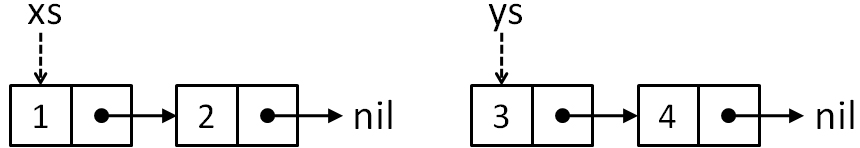
\includegraphics[width=7cm]{Lists.jpg}
\end{center}
{\em Copy this diagram}, and add to your drawing the list \verb!zs! defined by
\begin{verbatim}
zs = xs ++ ys
\end{verbatim}
Make sure that any sharing in the heap is shown accurately in your diagram.
\points{1}

\item
Study the following Haskell definitions, of the list reverse function
and a mysterious function:
\begin{verbatim}
reverse []     = []
reverse (x:xs) = reverse xs ++ [x]

mystery xs []     = xs
mystery xs (y:ys) = mystery (y:xs) ys
\end{verbatim}
In the following parts, assume that \verb!as! is a list of $m$
elements, and \verb!bs! is a list of $n$ elements.
\begin{enumerate}
\item
How many new cons cells are allocated during the evaluation of
\verb!as ++ bs!?
\points{1}
\item
How many cons cells are
allocated during the evaluation of \verb!reverse as!?
\points{1}
\item
How many cons cells are allocated during the evaluation of
\verb!mystery as bs!?
\points{1}
\item
What well-known compiler optimization is applicable to \verb!mystery!,
but not to \verb!reverse!?
\points{1}

\end{enumerate}
\item
QuickCheck properties take the form of boolean functions whose result
should always be true. For example,
\begin{verbatim}
prop_reverse xs =
  twice reverse xs == xs
\end{verbatim}
\begin{enumerate}
\item
What is the value of \verb!mystery [1,2] [3,4]!?
\points{1}
\item
Propose a QuickCheck property relating \verb!mystery!, \verb!reverse!
and \verb!(++)!.
\points{1}
\item
Give a more efficient definition of the \verb!reverse! function than
the one above, making use of \verb!mystery! in the definition.
\points{1}
\end{enumerate}

\item
The Haskell standard {\em higher-order function} \verb!foldl! is defined by
\begin{verbatim}
foldl f z []     = z
foldl f z (x:xs) = foldl f (f z x) xs
\end{verbatim}
Compare the definitions of \verb!foldl! and \verb!mystery!, and give
an alternative definition of \verb!mystery! in the form
\begin{verbatim}
mystery xs ys = foldl ...
\end{verbatim}
\points{2}

\end{enumerate}



\newpage
\section{Concurrency Oriented Programming [12 points]}

\begin{enumerate}
\item
How are Erlang data structures protected against simultaneous
modification by concurrent processes?
\points{1}

\item
Study the following code, which starts a server managing an integer value:
\begin{verbatim}
server() ->
    spawn(fun() -> server(0) end).

server(N) ->
    receive
        {read,Pid} ->
            Pid ! {self(),N},
            server(N);
        {write,New} ->
            server(New)
    end.
\end{verbatim}
Write the following functions for use in clients of the server:
\begin{enumerate}
\item
\verb!read(ServerPid)!, which returns the value \verb!N! currently managed by the server,
\points{1}
\item
\verb!write(ServerPid,New)!, which updates the value currently managed by the server to \verb!New!.
\points{1}
\end{enumerate}

\item
What value(s) can the following function return:
\begin{verbatim}
test() ->
    Server = server(),
    spawn(fun() -> write(Server,read(Server)+1) end),
    spawn(fun() -> write(Server,read(Server)+1) end),
    read(Server).
\end{verbatim}
\points{1}

\item
Extend the server to handle two new requests, to {\em lock} and {\em
  unlock} the server, such that the next request serviced after a {\em
  lock} must be an {\em unlock} request from the same client. Define
the following functions for use in clients:
\begin{enumerate}
\item
\verb!lock(ServerPid)!, which returns the value \verb!N! currently
managed by the server, and prevents any other request from being
serviced until
\points{1}
\item
\verb!unlock(ServerPid,New)!, which updates the value currently
managed by the server to \verb!New!, and permits other clients to use
the server again.
\points{1}
\end{enumerate}
Write the code which must be added to the \verb!server(N)! function to
handle these two new requests.
\points{2}
\item
What happens to requests sent to the server while it is locked by
another client?
\points{1}
\item
What happens (to the server and other clients) if a client crashes
after calling \verb!lock(Server)!, but before calling
\verb!unlock(Server,New)!?
\points{1}
\item
What is the effect of calling \verb!link(Pid)! in an Erlang process?
\points{1}
\item
How would you make the server {\em fault-tolerant}, so that if a
client crashes while holding the lock, then the server and other
clients are unaffected?  Show the code that you would add to the
\verb!server(N)! function.  \points{1}


\end{enumerate}


\newpage


\section{Logic Programming [12 points]}

\begin{enumerate}
\item
Given the three clauses
\begin{enumerate}
\item \verb!A || B!
\item \verb!C || D!
\item \verb?!A || D?
\end{enumerate}
state {\em which two} of the clauses can be combined using a resolution step, and give the resulting clause.
\points{1}

\item
For each pair of terms below, state whether the terms can be unified,
and if so, give the variable bindings that result. For example,
\verb!X! and \verb!2! {\em can} be unified, and the result is
\verb!X=2!.
\begin{enumerate}
\item \verb![X|Xs]! and \verb![1,2,3]!
\item \verb![X|Xs]! and \verb![]!
\item \verb!pair(A,y)! and \verb!pair(x,B)!
\item \verb!X! and \verb!Y!
\item \verb!pair(A,A)! and \verb!pair(B,C)!
\item \verb!pair(A,A)! and \verb!pair(b,c)!
\end{enumerate}
\points{3}

\item
Study the following Prolog program:
\begin{verbatim}
father(jack,robert).
father(robert,desmond).
father(robert,william).
mother(catherine,robert).
mother(mary,desmond).
mother(mary,william).
\end{verbatim}
What solutions will Prolog find for the following goals?
\begin{enumerate}
\item \verb!father(X,robert).!
\item \verb!father(robert,X).!
\end{enumerate}
\points{2}

\item
Extend the program above by defining a predicate \verb!parents(X,Y,Z)!
which holds if \verb!X! and \verb!Y! are the parents of \verb!Z!, and
\verb!X! is the father.
\points{1}

\item 
What solutions would Prolog find for the query \verb!parents(X,Y,Z)!?
\points{1}

\item
Study the following Prolog definitions:
\begin{verbatim}
append([],Ys,Ys).
append([X|Xs],Ys,[X|Zs]) :- append(Xs,Ys,Zs).
mystery([],[]).
mystery([X|Xs],Ys) :- mystery(Xs,Zs), append(Zs,[X],Ys).
\end{verbatim}
What solutions will Prolog find for the queries
\begin{enumerate}
\item \verb!mystery([1,2,3],X).!
\item \verb!mystery(X,[1,2,3]).!
\end{enumerate}
\points{2}

\item
One of the \verb!mystery! queries falls into an infinite loop after
printing the solutions. Which one?
\points{1}


\item
Rewrite the definition of \verb!mystery! to find the same solutions,
but so that neither of these queries falls into an infinite loop.
\points{1}

\end{enumerate}


\newpage
\section{Bonus Question on the Guest Lecture [1 point]}

Which application domain was Erlang first developed to address?
\begin{enumerate}
\item Scalable internet services.
\item Telecommunications.
\item Financial services.
\item Databases for cloud computing.
\end{enumerate}
\points{1}

\end{document}
